\documentclass[tikz, border=5, svgnames]{standalone}
\usepackage[utf8]{inputenc}
\usepackage[english]{babel}
\usepackage{xcolor}
\usepackage{amsmath}
\usepackage{amsfonts}
\usepackage{amssymb}
\usetikzlibrary{arrows.meta}

\usepackage{ifthen}
\begin{document}

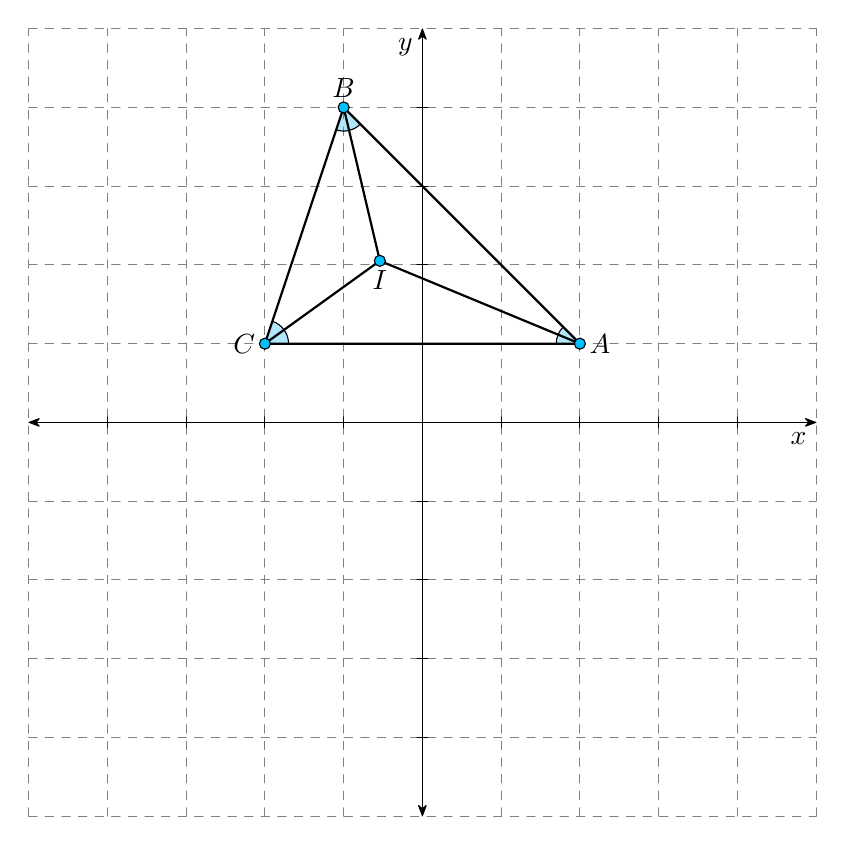
\begin{tikzpicture}

\draw[step=1cm,line width=0.4pt,line cap=round,xshift=0cm,yshift=0cm,Black!50,opacity=1,dashed,] (-5, -5) grid (5, 5);
\draw (5, 0) node [anchor= north east, ] {$x$};
\draw (0, 5) node [anchor= north east, ] {$y$};

    %axis
    \draw[{Stealth[round]}-{Stealth[round]},,] (-5,0) -- (5,0);
    \draw[{Stealth[round]}-{Stealth[round]},,] (0, -5) -- (0, 5);
	\foreach \x in {-4,...,4}
		\draw[line cap=round,] (\x*1, -2.0pt) -- (\x*1, 2.0pt);
	\foreach \y in {-4,...,4}
		\draw[line cap=round,] (-2.0pt, \y*1) -- (2.0pt, \y*1);

\fill[cyan, opacity=0.3] (-2, 1) -- ([shift=(0.0:0.3)]-2,1) arc[start angle=0.0, end angle=71.56505118, radius=0.3] -- cycle;
\draw  ([shift=(0.0:0.3)]-2,1) arc[start angle=0.0, end angle=71.56505118, radius=0.3];


\fill[cyan, opacity=0.3] (-1, 4) -- ([shift=(-108.43494882:0.3)]-1,4) arc[start angle=-108.43494882, end angle=-45.0, radius=0.3] -- cycle;
\draw  ([shift=(-108.43494882:0.3)]-1,4) arc[start angle=-108.43494882, end angle=-45.0, radius=0.3];


\fill[cyan, opacity=0.3] (2, 1) -- ([shift=(135.0:0.3)]2,1) arc[start angle=135.0, end angle=180.0, radius=0.3] -- cycle;
\draw  ([shift=(135.0:0.3)]2,1) arc[start angle=135.0, end angle=180.0, radius=0.3];


\draw[Black,opacity=1,solid,line cap=round,rounded corners=1pt,line width=0.8pt,]  (2, 1) -- (-1, 4) -- (-2, 1) -- cycle;
\draw[Black,opacity=1,solid,line cap=round,rounded corners=1pt,line width=0.8pt,]  (-0.54018151, 2.05217763) -- (2, 1);
\draw[Black,opacity=1,solid,line cap=round,rounded corners=1pt,line width=0.8pt,]  (-0.54018151, 2.05217763) -- (-1, 4);
\draw[Black,opacity=1,solid,line cap=round,rounded corners=1pt,line width=0.8pt,]  (-0.54018151, 2.05217763) -- (-2, 1);
\filldraw[line width=0.4pt, fill=DeepSkyBlue, draw=Black,opacity=1,] (2,1) circle (2pt);
\filldraw[line width=0.4pt, fill=DeepSkyBlue, draw=Black,opacity=1,] (-1,4) circle (2pt);
\filldraw[line width=0.4pt, fill=DeepSkyBlue, draw=Black,opacity=1,] (-2,1) circle (2pt);
\filldraw[line width=0.4pt, fill=DeepSkyBlue, draw=Black,opacity=1,] (-0.54018151,2.05217763) circle (2pt);
\draw (2, 1) node [anchor=west] {$A$};
\draw (-1, 4) node [anchor=south] {$B$};
\draw (-2, 1) node [anchor=east] {$C$};
\draw (-0.54018151, 2.05217763) node [anchor=north] {$I$};
\end{tikzpicture}
\end{document}
